% 学位论文 : 第二章 实验技术及设备简介
% 
% 更新记录:
%   {$LastChangedBy$}
%   {$LastChangedRevision$}
%   {$LastChangedDate$}

\chapter{实验技术及设备简介}
\section{生长设备}
<这类设备是干嘛的>
金属有机物气相外延沉积 

{\hei 金属有机化合物化学气相沉积}

金属有机化合物化学气相沉积简介

金属有机化合物化学气相沉积(MOCVD),参见图\ref{fig:mocvd},又称金属有机化合物气相外延(MOVPE)、有机金属化合物气相外延(OMVPE),他是利用金属有机化合物进行金属输运的一种气相外延生长技术。MOCVD适于生长薄层、超薄层,乃至超晶格、量子阱材料等低维结构,并且可以进行多片和大片的外延生长,易实现产业化。

MOCVD技术具有很多优点:
\begin{enumerate}[(1)]
\item 因为MOCVD可采用金属有机化合物(简称MO源)的种类很多,所以该方法具有制备多种化合物和多元固溶体的灵活性;
\item 生长外延层的各组分和掺杂剂都是以气态的方式通入反应室的,通过控制气态源的流量和通断时间可以控制外延层的组分、厚度、界面和掺杂浓度;
\item 通常情况下晶体生长速率与III族源的流量成正比,因此生长速率调节范围较广。
\end{enumerate}

MOCVD技术现已获得广泛应用,成为制备化合物半导体异质结、低维结构材料,以及生产化合物半导体光电子、微电子器件的重要方法。用MOCVD技术生产半导体激光器、发光管、太阳能电池和高频、高速电子器件等都已形成产业。
金属有机化合物化学气相沉积原理

\begin{figure}[h]
	\centering
	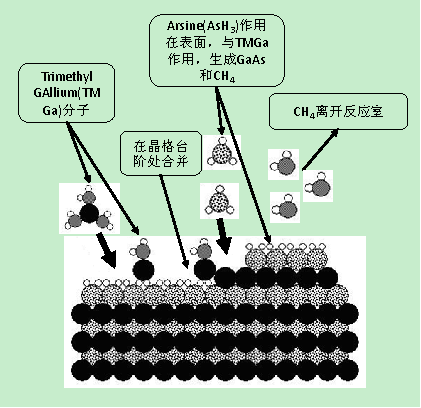
\includegraphics[width=0.8\textwidth]{ch02_MOCVD.pdf}
	\caption{MOCVD}
	\label{fig:mocvd}
\end{figure}

\section{表征设备}

<这类设备是干嘛的>

{\hei X-射线衍射仪} 这是一个我不知道是什么的设备,但听说它很有用,被用在了很多的领域,基本上实验室里的每一个实验都会用到这个设备,但它到底是做什么的呢,我是真的不知道,不过为了凑字我就只能写了这么长的一大串文字,总比粘一些不知道是啥的东西要好看多了。

{\hei 原子力显微镜}

{\hei 透射电镜}

{\hei 扫描电镜}

{\hei 腐蚀坑设备}

我来占个位置。\cite{BUPT_Thesis_Format_2004}

% 本章参考文献
\ifx\usechapbib\empty
\bibliographystyle{buptthesis}
\bibliography{bare_thesis}
\fi


%%% Local Variables: 
%%% mode: latex
%%% TeX-master: "bare_thesis"
%%% End: 
